\documentclass[10pt,letterpaper,journal]{IEEEtran}
\usepackage[T1]{fontenc}
\usepackage{amsmath,amsthm,amssymb,graphicx,booktabs,array,url}
\usepackage{newtxtext,newtxmath}
\usepackage{microtype}
\usepackage{cite}
\usepackage{balance}
\usepackage[hidelinks]{hyperref}
\usepackage{adjustbox}
\usepackage{placeins}
\setlength{\textwidth}{7in}
\setlength{\textheight}{9.5in}
\setlength{\oddsidemargin}{-0.25in}
\setlength{\evensidemargin}{-0.25in}
\setlength{\topmargin}{-0.80in}
\setlength{\columnsep}{0.30in}
\setlength{\parindent}{12pt}
\setlength{\parskip}{3pt}
\makeatletter
\def\ps@headings{\let\@oddhead\@empty\let\@evenhead\@empty%
\def\@oddfoot{\hfil\normalfont\fontsize{9}{10}\selectfont\thepage\hfil}%
\let\@evenfoot\@oddfoot}
\let\ps@IEEEtitlepagestyle\ps@headings
\makeatother
\pagestyle{headings}
\newtheorem{theorem}{Theorem}
\newtheorem{proposition}{Proposition}
\newtheorem{lemma}{Lemma}
\newtheorem{remark}{Remark}
\newtheorem{corollary}{Corollary}
\newtheorem{definition}{Definition}
\newcommand{\R}{\mathbb{R}}
\newcommand{\E}{\mathbb{E}}
\newcommand{\1}{\mathbf{1}}
\renewcommand{\thesection}{\arabic{section}}
\renewcommand{\thesubsection}{\thesection.\arabic{subsection}}
\renewcommand{\thesubsubsection}{\thesubsection.\arabic{subsubsection}}
\renewcommand{\thetable}{\arabic{table}}
% Auto-generated by gen_paper_assets.py; do not edit by hand.
\newcommand{\NCapePairDrop}{21}
\newcommand{\NCapeBreakDrop}{24}
\newcommand{\NCapePairP}{1.9\times10^{-6}}
\newcommand{\NCapeDiceCost}{0.007}
\newcommand{\NCapeClDiceCost}{0.012}
\newcommand{\NAurocOurs}{0.83}
\newcommand{\NAurocDet}{0.43}
\newcommand{\NAurocMC}{0.51}
\newcommand{\NAurocBN}{0.67}
\newcommand{\NCovConn}{0.899}
\newcommand{\NCovDisc}{0.899}
\newcommand{\NConfFlag}{12}
\newcommand{\NCRCRisk}{0.024}
\newcommand{\NCRCTrusted}{69}
\newcommand{\NCRCCaught}{72}
\newcommand{\NShiftUnw}{0.82}
\newcommand{\NShiftW}{0.98}
\newcommand{\NAnnFrac}{6.7}
\newcommand{\NClickGain}{0.087}
\newcommand{\NUncPairGain}{12}
\newcommand{\NUncPairP}{8.8\times10^{-5}}
\newcommand{\NDivClGain}{0.011}
\newcommand{\NDivClP}{3.8\times10^{-6}}
\newcommand{\NDivPairGain}{0.029}
\newcommand{\NDivPairP}{3.8\times10^{-6}}
\newcommand{\NSparseRatio}{99}
\newcommand{\NSamClGain}{0.043}
\newcommand{\NSamClP}{2.5\times10^{-8}}
\newcommand{\NSamBettiGain}{0.28}
\newcommand{\NSamBettiP}{7.1\times10^{-11}}
\newcommand{\NChainClGain}{0.058}
\newcommand{\NEnsAuroc}{0.914}
\newcommand{\NSingleAuroc}{0.878}
\newcommand{\NEnsFlag}{46}
\newcommand{\NSingleFlag}{90}
\newcommand{\NZSBase}{0.187}
\newcommand{\NZSBest}{0.391}
\newcommand{\NZSTexRaw}{0.297}
\newcommand{\NZSPolRaw}{0.167}
\newcommand{\NNRuns}{43}

\title{{\fontsize{17}{20}\selectfont\bfseries Conformal Connectivity: Calibrated, Provable Confidence\\ for Topology in Curvilinear Segmentation}}
\author{{\fontsize{11}{13}\selectfont Youssef Mourad}\\[3pt]
{\fontsize{10}{12}\selectfont\itshape Department of Artificial Intelligence Engineering, School of Engineering}\\
{\fontsize{10}{12}\selectfont\itshape University of Science and Technology at Zewail City}\\
{\fontsize{10}{12}\selectfont\itshape Giza, Egypt}\\
{\fontsize{10}{12}\selectfont Email: p-youssef.ramdan@zewailcity.edu.eg}\\
{\fontsize{10}{12}\selectfont ORCID: \href{https://orcid.org/0009-0002-7637-8862}{0009-0002-7637-8862}}}
\IEEEaftertitletext{%
\vspace{12pt}\par\noindent\hspace*{0.25in}\begin{minipage}{6.5in}
\fontsize{9}{12}\selectfont\noindent\textbf{\textit{Abstract---}} Topology-aware losses such as clDice and the connectivity-aware path enforcement loss CAPE make segmentations of vessels, neurons and roads more connected, but they still output a single binary map: nothing tells the user which connections can be trusted. We study connectivity itself as the object of uncertainty quantification. For a pair of points on a curvilinear structure we define the probability that they are connected, show that thresholded connectivity is governed by the widest-path (bottleneck) value of the probability map, and combine it with Monte-Carlo dropout into a connection score computed for thousands of pairs and hundreds of maps with a single three-dimensional connected-component labelling per tile. On retinal vessels (DRIVE, 3 seeds) the score detects topology errors with AUROC \NAurocOurs{}, against \NAurocDet{} for the thresholded prediction, \NAurocMC{} for MC-dropout alone and \NAurocBN{} for the bottleneck alone. Class-conditional split conformal prediction then attains coverage \NCovConn{}/\NCovDisc{} at a 0.90 target while flagging only \NConfFlag\% of connections, and an image-level conformal risk control theorem removes the within-image dependence of pairs: on CAPE models the expected fraction of wrongly auto-accepted connections is \NCRCRisk{} (bound 0.1) with \NCRCTrusted\% of connections trusted and \NCRCCaught\% of topology errors routed to a human. Covariate-shift weighting restores coverage when calibration and test images differ (\NShiftUnw{}$\to$\NShiftW{}). We use the same score to make CAPE label-efficient: scribbles are partial graphs on which CAPE applies unchanged, and yes/no connectivity questions chosen by the score with spatial diversity reach \NSparseRatio\% of the dense-label clDice with \NAnnFrac\% of pixels annotated, with \NUncPairGain\% fewer topology errors than random questions. Finally, a Segment-Anything model trained with CAPE (TopoSAM) gives significantly more connected few-shot road maps than a U-Net receiving the same clicks (clDice $+\NSamClGain$, $p=\NSamClP$). An independent re-evaluation confirms that CAPE reduces path-level topology errors by \NCapePairDrop\% ($p=\NCapePairP$). We report \NNRuns{} trained runs, paired tests and every negative result.\par\vspace{6pt}\noindent\textbf{\textit{Keywords---}} Topology-aware segmentation, uncertainty quantification, conformal prediction, conformal risk control, curvilinear structures, active learning, Segment Anything.\par\end{minipage}\hspace*{0.25in}\par\vspace{12pt}
}
\begin{document}
\maketitle

\section{Introduction}
\IEEEPARstart{C}{urvilinear} networks---retinal and cerebral vessels, neurons, road maps---are judged by their topology. A vessel segmentation with 99\% pixel accuracy is useless for blood-flow modelling if a single break disconnects a branch, and a road map with one false junction sends a router through a field. Topology-aware training objectives address this directly: clDice rewards centreline overlap \cite{cldice}, persistent-homology losses match Betti numbers \cite{hu2019,stucki2023}, and the recent connectivity-aware path enforcement loss CAPE penalises, along shortest paths sampled from the ground-truth graph, every break and every false connection \cite{cape}. These losses make predictions \emph{more} connected. They do not say \emph{which} predicted connections are correct.

That second question is the one a clinician or a map editor faces. Pixel-wise uncertainty maps \cite{gal2016,lakshminarayanan2017} are not the answer: a break is a single weak link in an otherwise confident vessel, and a pixel map shows no more than a faint dot there. Gupta et al.\ moved uncertainty to the level of topological structures \cite{gupta2023}, but without statistical guarantees. Conformal prediction gives distribution-free guarantees \cite{vovk2005,angelopoulos2021}, and has recently been applied to segmentation masks \cite{mossina2025}; to our knowledge it has not been applied to the question ``are these two points connected?''.

This paper makes connectivity the unit of uncertainty. Our contributions are:
\begin{enumerate}
\item a \emph{connection score}: thresholded connectivity is exactly a function of the widest-path value of the probability map (Proposition~\ref{prop:bottleneck}); averaging it over Monte-Carlo dropout samples gives a score that detects topology errors far better than either ingredient alone (Table~\ref{tab:scores}), with an implementation that answers every pair for every threshold and sample with one 3-D labelling per tile;
\item \emph{guarantees}: class-conditional split conformal sets with exact empirical coverage, an image-level conformal risk control theorem whose validity does not depend on the dependence of pairs inside an image (Theorem~\ref{th:crc}), and a covariate-shift-weighted variant for calibration data from a different distribution;
\item \emph{label-efficient CAPE}: scribbles are partial graphs, so CAPE applies to them unchanged; a new connectivity-click loss uses yes/no answers about point pairs, and the connection score with spatial diversity decides which pairs to ask;
\item \emph{TopoSAM}: a Segment-Anything model \cite{sam} with a frozen encoder, trained with CAPE and prompted by the same clicks, plus a study of zero-shot vessel-to-road transfer;
\item an exact parallel implementation of CAPE that is 7.5--14$\times$ faster, and an independent, path-level re-evaluation of CAPE itself;
\item a 3-seed evaluation with paired tests over \NNRuns{} trained runs, including all negative results.
\end{enumerate}
Section~\ref{sec:related} reviews related work, Section~\ref{sec:setup} defines connectivity and its error, Section~\ref{sec:score} the connection score, Section~\ref{sec:guar} the guarantees, Section~\ref{sec:label} label-efficient training, Section~\ref{sec:sam} TopoSAM. Section~\ref{sec:exp} reports experiments, Section~\ref{sec:disc} limitations and negative results, and Section~\ref{sec:impact} what changes in practice.

\begin{figure*}[t]
\centering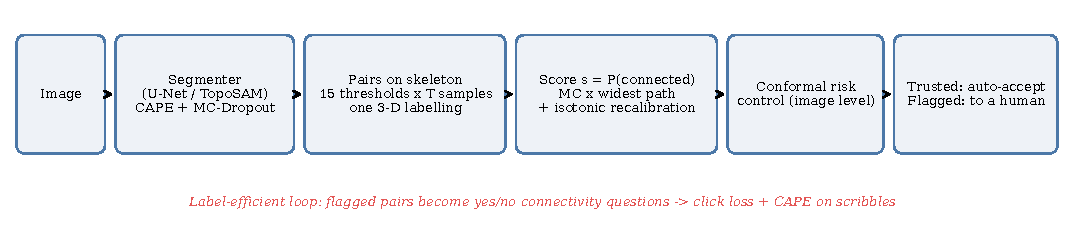
\includegraphics[width=0.98\textwidth]{figures/pipeline.pdf}
\caption{Conformal connectivity. A topology-aware segmenter is sampled with MC-dropout; for skeleton point pairs, connectivity is evaluated at 15 thresholds in every sample with one 3-D labelling per tile; the resulting connection score is recalibrated and turned into connection-level decisions with a conformal guarantee. Flagged pairs are shown to a human or, during training, become yes/no questions for label-efficient CAPE.}\label{fig:pipeline}
\end{figure*}

\section{Related Work}\label{sec:related}
\subsection{Topology-Aware Segmentation}
Pixel losses ignore connectivity, motivating losses on centrelines \cite{cldice}, persistence diagrams \cite{hu2019}, induced barcode matchings \cite{stucki2023}, perceptual features of thin structures \cite{mosinska2018}, region separation between neighbouring structures \cite{oner2022}, and shortest paths in the prediction \cite{cape}. CAPE \cite{cape} samples node pairs from the ground-truth graph, finds the cheapest path between them in the predicted distance or probability map with Dijkstra's algorithm \cite{dijkstra}, and penalises its cost, so both disconnections and false connections are penalised. It is the base of our work; we neither change its loss nor its sampling.

\subsection{Uncertainty for Segmentation and Topology}
MC-dropout \cite{gal2016} and deep ensembles \cite{lakshminarayanan2017} are standard epistemic estimators; post-hoc calibration uses temperature scaling \cite{guo2017} or isotonic regression \cite{zadrozny2002}. Topology-aware uncertainty \cite{gupta2023} estimates uncertainty per structure with discrete Morse theory; our unit is instead a pair of points and its connectivity, which is what a user verifies.

\subsection{Conformal Prediction}
Split conformal prediction gives finite-sample, distribution-free coverage under exchangeability \cite{vovk2005,angelopoulos2021}. Conformal risk control generalises coverage to any bounded monotone loss \cite{crc}; weighted conformal prediction handles covariate shift with likelihood ratios \cite{tibshirani2019}. For segmentation, morphological prediction sets \cite{mossina2025} give pixel-set guarantees. None of these address connectivity.

\subsection{Label-Efficient Delineation}
Mosinska et al.\ choose which parts of a delineation to annotate by the topological impact of errors \cite{mosinska2017}. Scribble supervision with size constraints \cite{kervadec2019} and random-convolution texture randomisation for domain generalisation \cite{randconv} are tools we reuse. Segment Anything \cite{sam} provides a promptable foundation model; we adapt it with CAPE.

\section{Connectivity and Its Error}\label{sec:setup}
Let $Y\subset\Omega$ be the ground-truth foreground of an image and $p:\Omega\to[0,1]$ a predicted probability map. Anchors are skeleton pixels of $Y$ subsampled on a $6\times6$ grid; a \emph{pair} $(u,v)$ is two anchors with $10\le\|u-v\|\le30$ pixels.

\begin{definition}[Local connectivity]
For a pair $(u,v)$ let $W(u,v)$ be the $64\times64$ tile of a stride-32 grid that contains both points, and $D(\cdot)$ the radius-2 disk. A set $S$ \emph{connects} $u$ and $v$ if one 8-connected component of $S\cap W$ meets both $D(u)$ and $D(v)$. The label is $y(u,v)=\1[Y \text{ connects } u,v]$ and the prediction at threshold $t$ is $c_t(u,v)=\1[\{p>t\}\text{ connects }u,v]$.
\end{definition}
Because $\|u-v\|\le30<32$, a containing tile always exists. A pair is a \emph{break} if $y=1,c_{0.5}=0$ and a \emph{merge} if $y=0,c_{0.5}=1$. The \emph{path topology error} of a prediction is the fraction of pairs with $c_{0.5}\ne y$. It complements Betti errors \cite{hu2019}: Betti numbers count components and holes, path error localises \emph{which} connections are wrong, which is what a reviewer must fix.

\section{The Connection Score}\label{sec:score}
\subsection{Connectivity is a Bottleneck Function}
\begin{proposition}[Widest path]\label{prop:bottleneck}
For a pair $(u,v)$ define the bottleneck value
\[b(u,v)=\max_{\pi:D(u)\leadsto D(v)\subset W}\ \min_{x\in\pi}p(x),\]
the maximum over 8-connected paths in the tile of the weakest probability along the path. Then $c_t(u,v)=\1[t<b(u,v)]$ for every $t\in[0,1)$. In particular $c_t$ is non-increasing in $t$.
\end{proposition}
\begin{proof}
If $t<b$, the maximising path $\pi$ has $p(x)\ge b>t$ for every $x\in\pi$, so $\pi\subset\{p>t\}$ joins $D(u)$ and $D(v)$ and $c_t=1$. Conversely, if $c_t=1$ there is a path in $\{p>t\}$; its minimum exceeds $t$, so $b>t$. Monotonicity follows because $\{p>t'\}\subseteq\{p>t\}$ for $t'\ge t$.
\end{proof}
The thresholded prediction therefore reveals only whether $b$ exceeds $0.5$. A real break has a bottleneck near zero; a faint but real capillary has a bottleneck of, say, 0.05--0.3, which plain thresholding and a linear threshold grid starting at 0.1 cannot distinguish. We evaluate $c_t$ on $L=15$ log-symmetric levels $\mathcal T=\{0.01,0.02,0.05,0.1,\dots,0.9,0.95,0.98,0.99\}$ and write
\[\mathrm{bn}(u,v)=\tfrac1L\textstyle\sum_{t\in\mathcal T}\1[t<b(u,v)],\]
a monotone step function of $b$ by Proposition~\ref{prop:bottleneck}.

\subsection{Epistemic Uncertainty of the Bottleneck}
With $T$ MC-dropout samples $p^{(1)},\dots,p^{(T)}$ \cite{gal2016}, the connection score is
\begin{equation}\label{eq:score}
s(u,v)=\frac1{TL}\sum_{k=1}^T\sum_{t\in\mathcal T}\1\big[t<b^{(k)}(u,v)\big],
\end{equation}
the average over the posterior samples and levels of the event ``the pair is connected''. MC-dropout alone ($s_{\rm mc}=\frac1T\sum_k\1[0.5<b^{(k)}]$) cannot see faint structures, and the bottleneck alone cannot see model uncertainty; \eqref{eq:score} uses both. Scores are mapped to probabilities by isotonic regression fitted on calibration pairs with the pool-adjacent-violators algorithm in $O(n\log n)$ \cite{zadrozny2002}; the map is monotone, so the conformal sets below do not change. The probability that the thresholded decision is wrong is $e=\hat P$ if $c_{0.5}=0$ and $1-\hat P$ otherwise; we use it to rank errors.

\subsection{All Pairs, Levels and Samples in One Labelling}
Evaluating \eqref{eq:score} naively needs one connected-component labelling per pair, level and sample. Instead, for each tile we stack the $M=1+L(T+1)$ binary maps (ground truth, the deterministic map and each MC sample at each level) into a volume and label it once with a structuring element that is 8-connected inside a slice and has no inter-slice connections, so labels never leak between maps. Each pair then reads its anchor labels in all $M$ slices at once. The cost is one labelling of $M\cdot64^2$ voxels per occupied tile, about one second per DRIVE image for 3,000 pairs and $M=316$. Thresholds are applied lazily per tile, so memory is $O(M\cdot64^2)$ rather than $O(M\cdot|\Omega|)$. Anchor pairs are found with a $k$-d tree in $O(n\log n)$.

\section{Guarantees}\label{sec:guar}
\subsection{Class-Conditional Split Conformal Prediction}
Non-conformity of label 1 is $1-s$ and of label 0 is $s$. For each class $c$, $q_c$ is the $\lceil(n_c+1)(1-\alpha)\rceil$-th smallest calibration non-conformity among pairs of class $c$, and $C(u,v)=\{c: a_c(u,v)\le q_c\}$. Singletons are automatic decisions; the pair is flagged otherwise.
\begin{proposition}[Mondrian coverage \cite{vovk2005}]\label{prop:mondrian}
If calibration and test pairs of class $c$ are exchangeable, $P(y\in C(u,v)\mid y=c)\ge1-\alpha$ for $c\in\{0,1\}$.
\end{proposition}
Class-conditional coverage matters: disconnected pairs are rare (about 13\% on DRIVE), and marginal coverage could be met while missing most of them. The weakness of Proposition~\ref{prop:mondrian} is its unit: pairs of one image share the same prediction and are not exchangeable with pairs of other images.

\subsection{Image-Level Conformal Risk Control}
We therefore guarantee a property of whole images. A connection is auto-accepted as connected if $s\ge\lambda_1$ and as disconnected if $s\le1-\lambda_0$; everything else is flagged. For image $i$ with $M_i$ pairs define
\begin{align*}
L_i^{1}(\lambda)&=\min\big(\#\{s\ge\lambda,\ y=0\}/M_i,\ B\big),\\
L_i^{0}(\lambda)&=\min\big(\#\{s\le1-\lambda,\ y=1\}/M_i,\ B\big),
\end{align*}
the fraction of the image's pairs that are wrongly auto-accepted on each side, capped at $B$.

\begin{theorem}[Image-level conformal risk control]\label{th:crc}
Let images $1,\dots,n+1$ be exchangeable, with no assumption on the pairs inside an image. For $j\in\{0,1\}$ let
\[\hat\lambda_j=\inf\Big\{\lambda:\ \tfrac{n}{n+1}\,\tfrac1n\textstyle\sum_{i\le n}L_i^{j}(\lambda)+\tfrac{B}{n+1}\le\tfrac\alpha2\Big\}.\]
Then $\E\big[L^1_{n+1}(\hat\lambda_1)+L^0_{n+1}(\hat\lambda_0)\big]\le\alpha$: in expectation, at most an $\alpha$ fraction of a new image's connections is wrongly auto-accepted (for losses below the cap).
\end{theorem}
\begin{proof}
Each $L_i^j$ is non-increasing and right-continuous in $\lambda$ and bounded by $B$, because raising $\lambda$ only removes auto-accepted pairs. Conformal risk control \cite{crc} then gives $\E[L^j_{n+1}(\hat\lambda_j)]\le\alpha/2$ for each side; the argument compares $\hat\lambda_j$ with the oracle threshold computed from all $n+1$ exchangeable losses and bounds the unknown test loss by $B$. Summing the two sides gives the claim. Exchangeability is required only between images, so the dependence of pairs inside an image is irrelevant.
\end{proof}
\begin{remark}[Feasibility]
A threshold exists only if $\alpha/2>B/(n+1)$. With $n=16$ calibration images and $B=0.5$ this is $\alpha>0.059$; below it the method correctly trusts nothing (Fig.~\ref{fig:crc}). We choose $B=0.5$ a priori; in all experiments the cap never binds.
\end{remark}

\subsection{Calibration Under Covariate Shift}
When calibration images come from a different distribution (e.g., held-out training images rather than test-like images), we estimate the likelihood ratio $w(x)=dP_{\rm test}/dP_{\rm cal}$ with a logistic domain classifier on pair features (the four scores and two image-level summaries; quadratic features), trained to separate calibration pairs from \emph{unlabelled} test pairs, and use weighted conformal prediction \cite{tibshirani2019}: label $c$ enters the set iff the calibration weight of class-$c$ non-conformities strictly below the test value is less than $(1-\alpha)(W_c+w(x))$. With one cumulative sum and a binary search this costs $O((n+m)\log n)$ for all test pairs.

\section{Label-Efficient CAPE}\label{sec:label}
CAPE needs the ground-truth graph only to sample paths. A scribble drawn along a vessel centreline is a subgraph of that graph, so CAPE applies to scribbles unchanged; we skeletonise the scribble masks and feed them to the loss as ground truth. Pixel supervision is a class-balanced partial cross-entropy on scribbled pixels, plus a size constraint \cite{kervadec2019}
\[\mathcal L_{\rm size}=\big[(\ell-\bar p)_+\big]^2+\big[(\bar p-h)_+\big]^2,\]
where $\bar p$ is the mean predicted probability in the field of view and $[\ell,h]$ a loose prior band ($[0.08,0.16]$ for vessels, $[0.02,0.08]$ for roads). Background strokes are cheap to draw, so they receive five times the positive budget. Without the size constraint and the denser background strokes, scribble-only training reached Dice 0.41 in a pilot run.

\textbf{Connectivity clicks.} An annotator is shown two points and answers \emph{connected}, \emph{not connected} or \emph{not a vessel}. Let $\pi^\star$ be the cheapest path between the clicks under cost $1-p$ (Dijkstra, no corridor because no ground-truth path is known). The click loss is
\begin{align*}
\mathcal L_{\rm yes}&=\tfrac1{|\pi^\star|}\textstyle\sum_{x\in\pi^\star}(1-p(x))^2,\\
\mathcal L_{\rm no}&=\tfrac1k\textstyle\sum_{x\in\mathcal W_k(\pi^\star)}p(x)^2,
\end{align*}
where $\mathcal W_k$ are the $k=3$ weakest pixels of $\pi^\star$: a connected pair must be joined by vessel, and a disconnected pair needs only one gap, which should form at its weakest links. ``Not a vessel'' answers become negative clicks.

\textbf{Which pairs to ask.} Candidate pairs lie on the skeleton of $\{p>0.3\}$. Their connection score \eqref{eq:score} is computed from the current model; pairs are ranked by $|2s-1|$ and selected greedily with spatial non-maximum suppression (no two selected midpoints closer than $r$ pixels, $k$-d tree, $O(n\log n)$), so the budget is not spent on redundant questions about one gap. The radius is chosen on the validation images only.

\section{TopoSAM}\label{sec:sam}
TopoSAM keeps the ViT-B image encoder of Segment Anything \cite{sam} frozen and caches its embeddings once per image and augmentation, so training runs only the prompt encoder, the mask decoder and a small high-resolution refiner (a 3-level U-Net with MC-dropout that predicts a residual on top of SAM's upsampled logit). SAM's $256\times256$ output cannot draw one-pixel vessels; the refiner can. Prompts are 5--20 positive and negative clicks drawn from scribbles; at test time 10+10. The model is trained with CAPE and a pixel loss, on dense labels (vessels) or scribbles only (roads). For domain generalisation we add inverted-intensity copies and random-convolution textures \cite{randconv} as further cached embedding variants.

\textbf{Exact parallel CAPE.} In CAPE the path search is not differentiated; only the cost along the selected path is. We therefore run the official path sampling and Dijkstra search \cite{cape} in torch-free worker processes that return integer coordinates, and evaluate the cost with one gather on the GPU. On identical seeds the loss equals the official implementation to $10^{-5}$ and is 7.5--14$\times$ faster on our machine.

\section{Experiments}\label{sec:exp}
\subsection{Setup}
\textbf{Data.} DRIVE \cite{drive}: 20 training images (16 for training, 4 held out for validation), 20 test images. Massachusetts Roads \cite{mnih2013}: central $1024^2$ crops of the evaluation tiles, 40 tiles for few-shot training, 20 for calibration, 60 for testing.
\textbf{Models.} U-Net \cite{unet} with 7.8\,M parameters and spatial dropout 0.2 in the bottleneck and decoder, AdamW with a one-cycle schedule, $256^2$ crops, 6,000 iterations. Following the CAPE authors, CAPE fine-tunes the converged pixel-loss model (2,000 iterations). MC-dropout uses $T=20$ samples (10 on roads).
\textbf{Protocol.} Every configuration is trained with 3 seeds; tables report mean\,$\pm$\,std over seeds. Comparisons use a two-sided Wilcoxon signed-rank test \cite{wilcoxon} over test images on seed-averaged values, and count the seeds in which the difference has the same sign. Conformal results use random image-level calibration/test splits (100 or 50 repetitions). Scribbles and connectivity answers are simulated from the ground truth. All experiments ran on a single 8\,GB laptop GPU.

% Auto-generated by gen_paper_assets.py; do not edit by hand.
\begin{table*}[t]
\centering\caption{Segmentation and topology on the 20 DRIVE test images (U-Net, 3 seeds, mean\,$\pm$\,std over seeds). Path err.\ is the fraction of point pairs whose connectivity differs from the ground truth; it splits into breaks (connected in truth, disconnected in prediction) and merges.}\label{tab:seg}
\footnotesize\begin{tabular}{lcccccc}\toprule
Training loss & Dice$\uparrow$ & clDice$\uparrow$ & $\beta_0$ err.$\downarrow$ & Path err.$\downarrow$ & Breaks$\downarrow$ & Merges$\downarrow$\\\midrule
BCE+Dice & 0.825\,$\pm$\,0.001 & 0.830\,$\pm$\,0.001 & 1.043\,$\pm$\,0.096 & 0.227\,$\pm$\,0.004 & 0.215\,$\pm$\,0.005 & 0.012\,$\pm$\,0.001\\
+ clDice \cite{cldice} & 0.820\,$\pm$\,0.001 & 0.843\,$\pm$\,0.000 & 0.742\,$\pm$\,0.013 & 0.215\,$\pm$\,0.008 & 0.203\,$\pm$\,0.007 & 0.012\,$\pm$\,0.001\\
+ CAPE \cite{cape} & 0.818\,$\pm$\,0.001 & 0.817\,$\pm$\,0.001 & 1.044\,$\pm$\,0.024 & 0.179\,$\pm$\,0.002 & 0.162\,$\pm$\,0.002 & 0.016\,$\pm$\,0.001\\
\bottomrule\end{tabular}\end{table*}


\subsection{CAPE Reduces Path-Level Topology Errors}
Table~\ref{tab:seg} re-evaluates the three losses with the path error of Section~\ref{sec:setup}. CAPE reduces path errors by \NCapePairDrop\% and breaks by \NCapeBreakDrop\% relative to BCE+Dice ($p=\NCapePairP$, all seeds), independently confirming the claim of \cite{cape} with a different metric. It costs \NCapeDiceCost{} Dice and \NCapeClDiceCost{} clDice, both significant (Table~\ref{tab:tests}). clDice gives the fewest components ($\beta_0$) but a smaller path-error reduction: the two losses repair different failures.

% Auto-generated by gen_paper_assets.py; do not edit by hand.
\begin{table*}[t]
\centering\caption{Which connection score detects topology errors? AUROC of the error score and expected calibration error after isotonic recalibration, per training loss; 3 seeds $\times$ 50 random image-level 10/10 calibration/test splits.}\label{tab:scores}
\footnotesize\begin{adjustbox}{max width=\textwidth}\begin{tabular}{lcccccc}\toprule
 & \multicolumn{3}{c}{AUROC(error)$\uparrow$} & \multicolumn{3}{c}{ECE$\downarrow$}\\\cmidrule(lr){2-4}\cmidrule(lr){5-7}
Score & Dice & clDice & CAPE & Dice & clDice & CAPE\\\midrule
Threshold at 0.5 & 0.426\,$\pm$\,0.033 & 0.407\,$\pm$\,0.029 & 0.387\,$\pm$\,0.013 & 0.167\,$\pm$\,0.012 & 0.161\,$\pm$\,0.002 & 0.154\,$\pm$\,0.013\\
MC-Dropout only & 0.511\,$\pm$\,0.027 & 0.468\,$\pm$\,0.011 & 0.553\,$\pm$\,0.003 & 0.136\,$\pm$\,0.005 & 0.138\,$\pm$\,0.002 & 0.104\,$\pm$\,0.003\\
Bottleneck only & 0.669\,$\pm$\,0.016 & 0.641\,$\pm$\,0.033 & 0.633\,$\pm$\,0.018 & 0.094\,$\pm$\,0.003 & 0.097\,$\pm$\,0.007 & 0.083\,$\pm$\,0.003\\
MC $\times$ bottleneck (ours) & 0.827\,$\pm$\,0.023 & 0.839\,$\pm$\,0.047 & 0.741\,$\pm$\,0.016 & 0.053\,$\pm$\,0.008 & 0.045\,$\pm$\,0.013 & 0.061\,$\pm$\,0.003\\
\bottomrule\end{tabular}\end{adjustbox}\end{table*}

\begin{figure}[t]
\centering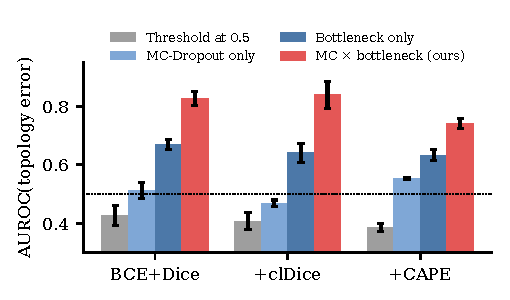
\includegraphics[width=\columnwidth]{figures/scores.pdf}
\caption{Error detection by connection score (3 seeds). Only the combination of MC-dropout and the bottleneck detects topology errors reliably; thresholding is worse than chance because its few errors are confident.}\label{fig:scores}
\end{figure}

\subsection{The Connection Score Detects Topology Errors}
Table~\ref{tab:scores} and Fig.~\ref{fig:scores} compare four scores. The thresholded decision has AUROC below 0.5: when it is wrong it is confidently wrong. MC-dropout alone is near chance, because it varies the prediction only near 0.5 and breaks sit far below. The bottleneck alone sees faint structures (AUROC \NAurocBN). Their combination reaches \NAurocOurs{} on the Dice model and also the lowest calibration error. CAPE models are harder to diagnose (AUROC 0.74): CAPE makes predictions more connected and more confident, which is an argument for, not against, attaching connection-level confidence to it.

% Auto-generated by gen_paper_assets.py; do not edit by hand.
\begin{table*}[t]
\centering\caption{Guarantees at $\alpha=0.1$ (3 seeds). Left: class-conditional split conformal prediction (target coverage $\ge 0.90$ per class). Right: image-level conformal risk control (target: expected wrongly auto-accepted fraction per image $\le 0.10$). Random image-level splits (DRIVE 16/4 for CRC, 10/10 for conformal; roads 40/40).}\label{tab:guar}
\footnotesize\begin{tabular}{lcccccc}\toprule
 & \multicolumn{3}{c}{Mondrian conformal} & \multicolumn{3}{c}{Image-level CRC}\\\cmidrule(lr){2-4}\cmidrule(lr){5-7}
Model & Cov. conn. & Cov. disc. & Flagged$\downarrow$ & Risk ($\le$0.1) & Trusted$\uparrow$ & Errors flagged$\uparrow$\\\midrule
DRIVE, BCE+Dice & 0.899\,$\pm$\,0.001 & 0.899\,$\pm$\,0.001 & 0.12\,$\pm$\,0.00 & 0.024\,$\pm$\,0.001 & 0.68\,$\pm$\,0.00 & 0.59\,$\pm$\,0.02\\
DRIVE, clDice & 0.900\,$\pm$\,0.001 & 0.899\,$\pm$\,0.001 & 0.13\,$\pm$\,0.01 & 0.034\,$\pm$\,0.007 & 0.71\,$\pm$\,0.02 & 0.62\,$\pm$\,0.01\\
DRIVE, CAPE & 0.899\,$\pm$\,0.001 & 0.899\,$\pm$\,0.001 & 0.12\,$\pm$\,0.00 & 0.024\,$\pm$\,0.001 & 0.69\,$\pm$\,0.00 & 0.72\,$\pm$\,0.02\\
DRIVE, scribbles + clicks & 0.931\,$\pm$\,0.016 & 0.898\,$\pm$\,0.002 & 0.35\,$\pm$\,0.04 & 0.022\,$\pm$\,0.001 & 0.56\,$\pm$\,0.01 & 0.85\,$\pm$\,0.02\\
Roads, U-Net few-shot & 0.902\,$\pm$\,0.001 & 0.890\,$\pm$\,0.002 & 0.31\,$\pm$\,0.02 & 0.076\,$\pm$\,0.001 & 0.84\,$\pm$\,0.00 & 0.49\,$\pm$\,0.03\\
Roads, TopoSAM few-shot & 0.907\,$\pm$\,0.009 & 0.977\,$\pm$\,0.024 & 0.84\,$\pm$\,0.06 & 0.039\,$\pm$\,0.001 & 0.72\,$\pm$\,0.03 & 0.83\,$\pm$\,0.00\\
\bottomrule\end{tabular}\end{table*}

\begin{figure}[t]
\centering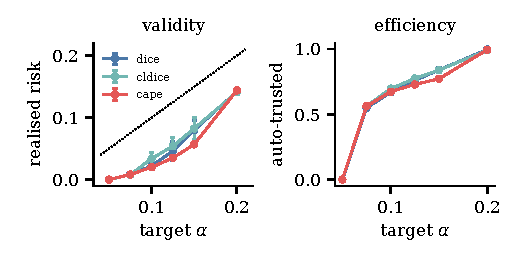
\includegraphics[width=\columnwidth]{figures/crc.pdf}
\caption{Image-level conformal risk control on DRIVE (3 seeds per loss). Left: realised risk stays below the target $\alpha$ (dotted). Right: fraction of connections auto-accepted. Below $\alpha\approx0.06$ the bound $B/(n+1)$ makes the problem infeasible and nothing is trusted.}\label{fig:crc}
\end{figure}

\subsection{Guarantees}
Table~\ref{tab:guar} shows that the class-conditional sets attain coverage \NCovConn{}/\NCovDisc{} for a 0.90 target with a standard deviation of about 0.001 over seeds, flagging \NConfFlag\% of connections on DRIVE. Image-level CRC keeps the expected wrongly-accepted fraction at \NCRCRisk{} on CAPE models while auto-accepting \NCRCTrusted\% of connections; the \NCRCCaught\% of topology errors that it flags are exactly where a reviewer should look. Fig.~\ref{fig:crc} confirms validity for every $\alpha$. Under distribution shift (Table~\ref{tab:shift}) the unweighted guarantee fails (coverage of connected pairs \NShiftUnw{} for a 0.90 target); weighting restores it (\NShiftW) at the price of flagging more connections---the honest response when the calibration data are known to differ. On roads, weighting changes nothing: the effective sample size equals the number of pairs, i.e.\ the road tiles differ in $P(y\mid x)$ rather than in $x$, which no covariate correction can fix; random tile-level calibration is then required.

% Auto-generated by gen_paper_assets.py; do not edit by hand.
\begin{table}[t]
\centering\caption{Calibration under distribution shift (seed 0): calibrating on held-out \emph{training} images breaks coverage of connected pairs; covariate-shift weighting with a domain classifier on unlabelled test pairs restores it ($\alpha=0.1$).}\label{tab:shift}
\setlength{\tabcolsep}{2pt}\scriptsize\begin{tabular}{lccccc}\toprule
 & \multicolumn{2}{c}{Unweighted} & \multicolumn{2}{c}{Weighted (ours)} & \\\cmidrule(lr){2-3}\cmidrule(lr){4-5}
Model & conn. & disc. & conn. & disc. & Flagged\\\midrule
DRIVE, BCE+Dice & 0.820 & 0.934 & 0.940 & 0.948 & 0.07 $\to$ 0.48\\
DRIVE, clDice & 0.819 & 0.940 & 0.936 & 0.947 & 0.08 $\to$ 0.45\\
DRIVE, CAPE & 0.818 & 0.939 & 0.977 & 0.975 & 0.05 $\to$ 0.72\\
\bottomrule\end{tabular}\end{table}

\begin{figure*}[t]
\centering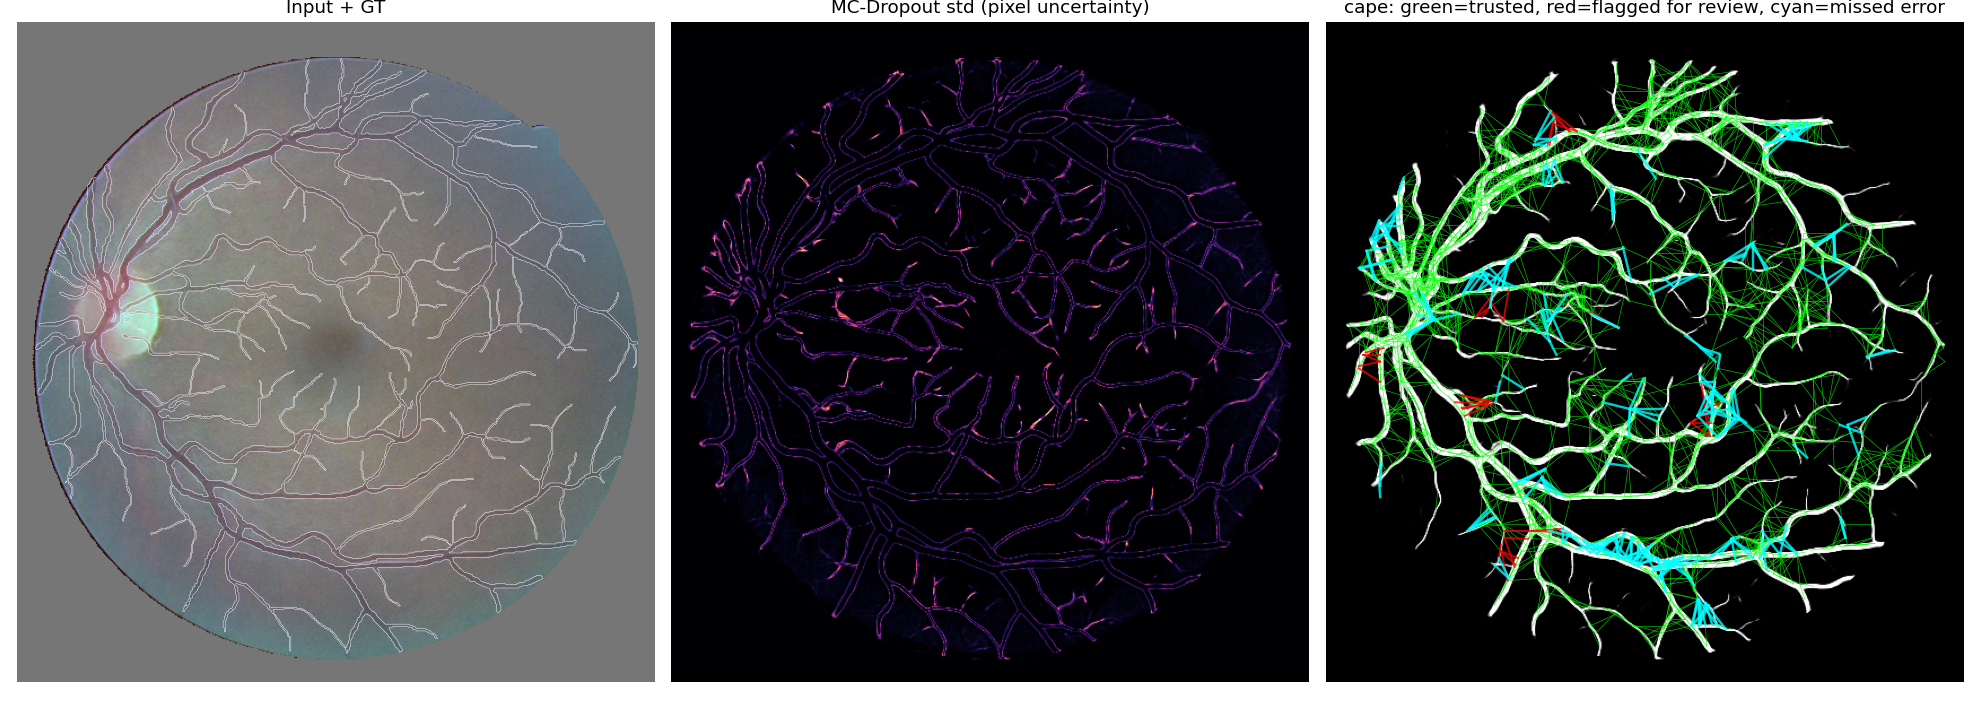
\includegraphics[width=0.85\textwidth]{figures/qual_drive.png}
\caption{A DRIVE test image with the CAPE model. Left: input and ground truth. Middle: MC-dropout standard deviation. Right: every tested connection, green if auto-accepted correctly, red if flagged for review, cyan if auto-accepted wrongly ($\alpha=0.1$, class-conditional sets). Errors and flags concentrate at the optic disc and thin capillaries.}\label{fig:qual}
\end{figure*}

% Auto-generated by gen_paper_assets.py; do not edit by hand.
\begin{table*}[t]
\centering\caption{Label-efficient CAPE on DRIVE (3 seeds). All variants use scribbles on 10\% of the vessel length (6.7\% of FOV pixels touched); click variants add $2\times40$ yes/no connectivity questions per image. No dense label is used for training or model selection. The noisy annotator shifts every stroke by up to 2\,px and answers 10\% of questions wrongly.}\label{tab:label}
\footnotesize\begin{tabular}{lcccccc}\toprule
Supervision & Dice$\uparrow$ & clDice$\uparrow$ & $\beta_0$ err.$\downarrow$ & Path err.$\downarrow$ & Breaks$\downarrow$ & Merges$\downarrow$\\\midrule
Scribbles + CAPE & 0.636\,$\pm$\,0.029 & 0.710\,$\pm$\,0.015 & 1.029\,$\pm$\,0.079 & 0.470\,$\pm$\,0.028 & 0.454\,$\pm$\,0.029 & 0.016\,$\pm$\,0.002\\
+ random connectivity clicks & 0.700\,$\pm$\,0.002 & 0.797\,$\pm$\,0.003 & 1.003\,$\pm$\,0.035 & 0.339\,$\pm$\,0.017 & 0.324\,$\pm$\,0.018 & 0.015\,$\pm$\,0.001\\
+ uncertainty clicks & 0.690\,$\pm$\,0.003 & 0.791\,$\pm$\,0.005 & 0.904\,$\pm$\,0.011 & 0.299\,$\pm$\,0.016 & 0.271\,$\pm$\,0.016 & 0.027\,$\pm$\,0.002\\
+ unc.\ + diversity ($r$=24) & 0.701\,$\pm$\,0.001 & 0.807\,$\pm$\,0.001 & 0.976\,$\pm$\,0.027 & 0.304\,$\pm$\,0.014 & 0.285\,$\pm$\,0.016 & 0.019\,$\pm$\,0.002\\
+ unc.\ + diversity ($r$=48, val.) & 0.700\,$\pm$\,0.000 & 0.808\,$\pm$\,0.001 & 0.932\,$\pm$\,0.033 & 0.311\,$\pm$\,0.011 & 0.293\,$\pm$\,0.012 & 0.018\,$\pm$\,0.001\\
same, noisy annotator & 0.619\,$\pm$\,0.013 & 0.734\,$\pm$\,0.008 & 1.087\,$\pm$\,0.035 & 0.445\,$\pm$\,0.017 & 0.426\,$\pm$\,0.018 & 0.019\,$\pm$\,0.001\\
\midrule Dense labels + CAPE (ref.) & 0.818\,$\pm$\,0.001 & 0.817\,$\pm$\,0.001 & 1.044\,$\pm$\,0.024 & 0.179\,$\pm$\,0.002 & 0.162\,$\pm$\,0.002 & 0.016\,$\pm$\,0.001\\
\bottomrule\end{tabular}\end{table*}

\begin{figure}[t]
\centering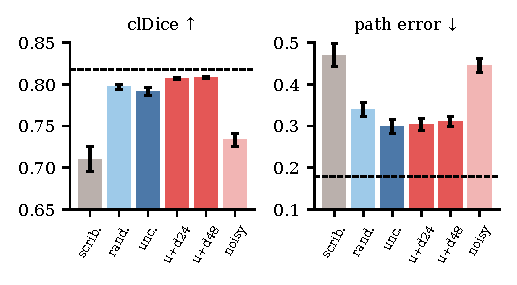
\includegraphics[width=\columnwidth]{figures/label_efficiency.pdf}
\caption{Label-efficient CAPE (3 seeds). Dashed: CAPE trained on dense labels. Uncertainty-chosen questions with spatial diversity (red) are best on both clDice and path error among the sparse variants.}\label{fig:label}
\end{figure}

\subsection{Label-Efficient CAPE}
Table~\ref{tab:label} and Fig.~\ref{fig:label} show that connectivity clicks add $+\NClickGain$ clDice over scribbles alone. Choosing the questions with the connection score reduces topology errors by a further \NUncPairGain\% ($p=\NUncPairP$), mainly breaks, but alone it loses a little clDice: top-ranked uncertain pairs cluster around the same gaps. Adding spatial diversity removes this trade-off: against random questions it gains $+\NDivClGain$ clDice ($p=\NDivClP$) \emph{and} $\NDivPairGain$ path error ($p=\NDivPairP$) in all seeds. With \NAnnFrac\% of pixels annotated it reaches \NSparseRatio\% of the dense-label clDice, although its path error remains clearly higher than with dense labels. The phase-1 guarantees carry over to these weakly supervised models (Table~\ref{tab:guar}). With a noisy annotator---every stroke displaced by up to 2\,px, so that 44\% of positive scribble pixels miss the vessel, and 10\% of answers wrong---performance drops substantially but remains better than clean scribble-only training (Table~\ref{tab:tests}).

% Auto-generated by gen_paper_assets.py; do not edit by hand.
\begin{table}[t]
\centering\caption{Paired comparisons: difference of seed means, two-sided Wilcoxon signed-rank $p$ over test images (seed-averaged), and the number of seeds in which A is better.}\label{tab:tests}
\setlength{\tabcolsep}{2pt}\scriptsize\begin{tabular}{llrrc}\toprule
A vs B & Metric & $\Delta$ & $p$ & Seeds\\\midrule
CAPE vs BCE+Dice & path err. & -0.048 & $1.9\times10^{-6}$ & 3/3\\
CAPE vs BCE+Dice & clDice & -0.012 & $1.0\times10^{-4}$ & 0/3\\
random clicks vs scribbles & clDice & +0.087 & $1.9\times10^{-6}$ & 3/3\\
unc.\ clicks vs random & path err. & -0.041 & $8.8\times10^{-5}$ & 3/3\\
unc.+div.\ vs random & clDice & +0.011 & $3.8\times10^{-6}$ & 3/3\\
unc.+div.\ vs random & path err. & -0.029 & $3.8\times10^{-6}$ & 3/3\\
noisy unc.+div.\ vs clean scribbles & clDice & +0.023 & $3.8\times10^{-6}$ & 3/3\\
TopoSAM vs click U-Net & clDice & +0.043 & $2.5\times10^{-8}$ & 3/3\\
TopoSAM vs click U-Net & $\beta_0$ err. & -0.280 & $7.1\times10^{-11}$ & 3/3\\
TopoSAM vs click U-Net & path err. & +0.002 & $0.935$ & 1/3\\
init.\ DRIVE vs init.\ SAM & clDice & +0.058 & $2.2\times10^{-9}$ & 3/3\\
RandConv init.\ vs DRIVE init. & clDice & -0.018 & $2.7\times10^{-5}$ & 0/3\\
\bottomrule\end{tabular}\end{table}

% Auto-generated by gen_paper_assets.py; do not edit by hand.
\begin{table*}[t]
\centering\caption{Few-shot road extraction (Massachusetts Roads, 40 training tiles with scribbles only, 60 test tiles, 3 seeds). TopoSAM and the click U-Net receive the same 10+10 click prompts. CRC trusted: fraction of connections auto-accepted at risk $\le0.1$.}\label{tab:roads}
\footnotesize\begin{tabular}{lcccccc}\toprule
Model & Dice$\uparrow$ & clDice$\uparrow$ & $\beta_0$ err.$\downarrow$ & Path err.$\downarrow$ & AUROC(err)$\uparrow$ & CRC trusted$\uparrow$\\\midrule
U-Net + CAPE & 0.554\,$\pm$\,0.025 & 0.637\,$\pm$\,0.033 & 0.794\,$\pm$\,0.163 & 0.252\,$\pm$\,0.010 & 0.942\,$\pm$\,0.001 & 0.83\,$\pm$\,0.01\\
U-Net + CAPE + same clicks & 0.566\,$\pm$\,0.018 & 0.638\,$\pm$\,0.025 & 0.899\,$\pm$\,0.263 & 0.224\,$\pm$\,0.013 & 0.940\,$\pm$\,0.001 & 0.84\,$\pm$\,0.00\\
TopoSAM, init.\ SAM & 0.495\,$\pm$\,0.007 & 0.624\,$\pm$\,0.004 & 1.005\,$\pm$\,0.054 & 0.216\,$\pm$\,0.002 & 0.884\,$\pm$\,0.009 & 0.69\,$\pm$\,0.03\\
TopoSAM, init.\ DRIVE (ours) & 0.551\,$\pm$\,0.012 & 0.682\,$\pm$\,0.019 & 0.619\,$\pm$\,0.077 & 0.227\,$\pm$\,0.005 & 0.887\,$\pm$\,0.019 & 0.72\,$\pm$\,0.03\\
TopoSAM, init.\ DRIVE-RandConv & 0.545\,$\pm$\,0.009 & 0.664\,$\pm$\,0.013 & 0.691\,$\pm$\,0.060 & 0.229\,$\pm$\,0.008 & 0.879\,$\pm$\,0.011 & 0.71\,$\pm$\,0.02\\
\bottomrule\end{tabular}\end{table*}


\subsection{TopoSAM and Road Extraction}
On DRIVE with dense labels TopoSAM matches the U-Net (Dice 0.820 vs.\ 0.818 for seed 0) although its encoder is frozen. On roads (Table~\ref{tab:roads}, Fig.~\ref{fig:roads}), the fair baseline is a U-Net that receives the same click prompts as input heat maps. TopoSAM is significantly more connected: clDice $+\NSamClGain$ ($p=\NSamClP$) and $\NSamBettiGain$ fewer components per patch ($p=\NSamBettiP$), in all seeds. It is not uniformly better: it loses 0.015 Dice and produces more merges, and the path error is a tie. Initialising TopoSAM from the vessel-trained model instead of plain SAM adds $+\NChainClGain$ clDice. Connection-level uncertainty transfers to roads (AUROC 0.88--0.94), but a single TopoSAM gives uninformative class-conditional sets; prompt resampling plus a three-member decoder ensemble raises AUROC from \NSingleAuroc{} to \NEnsAuroc{} and lowers the flagged fraction from \NSingleFlag\% to \NEnsFlag\%, while image-level CRC is efficient even for a single model (72\% trusted).

\begin{figure*}[t]
\centering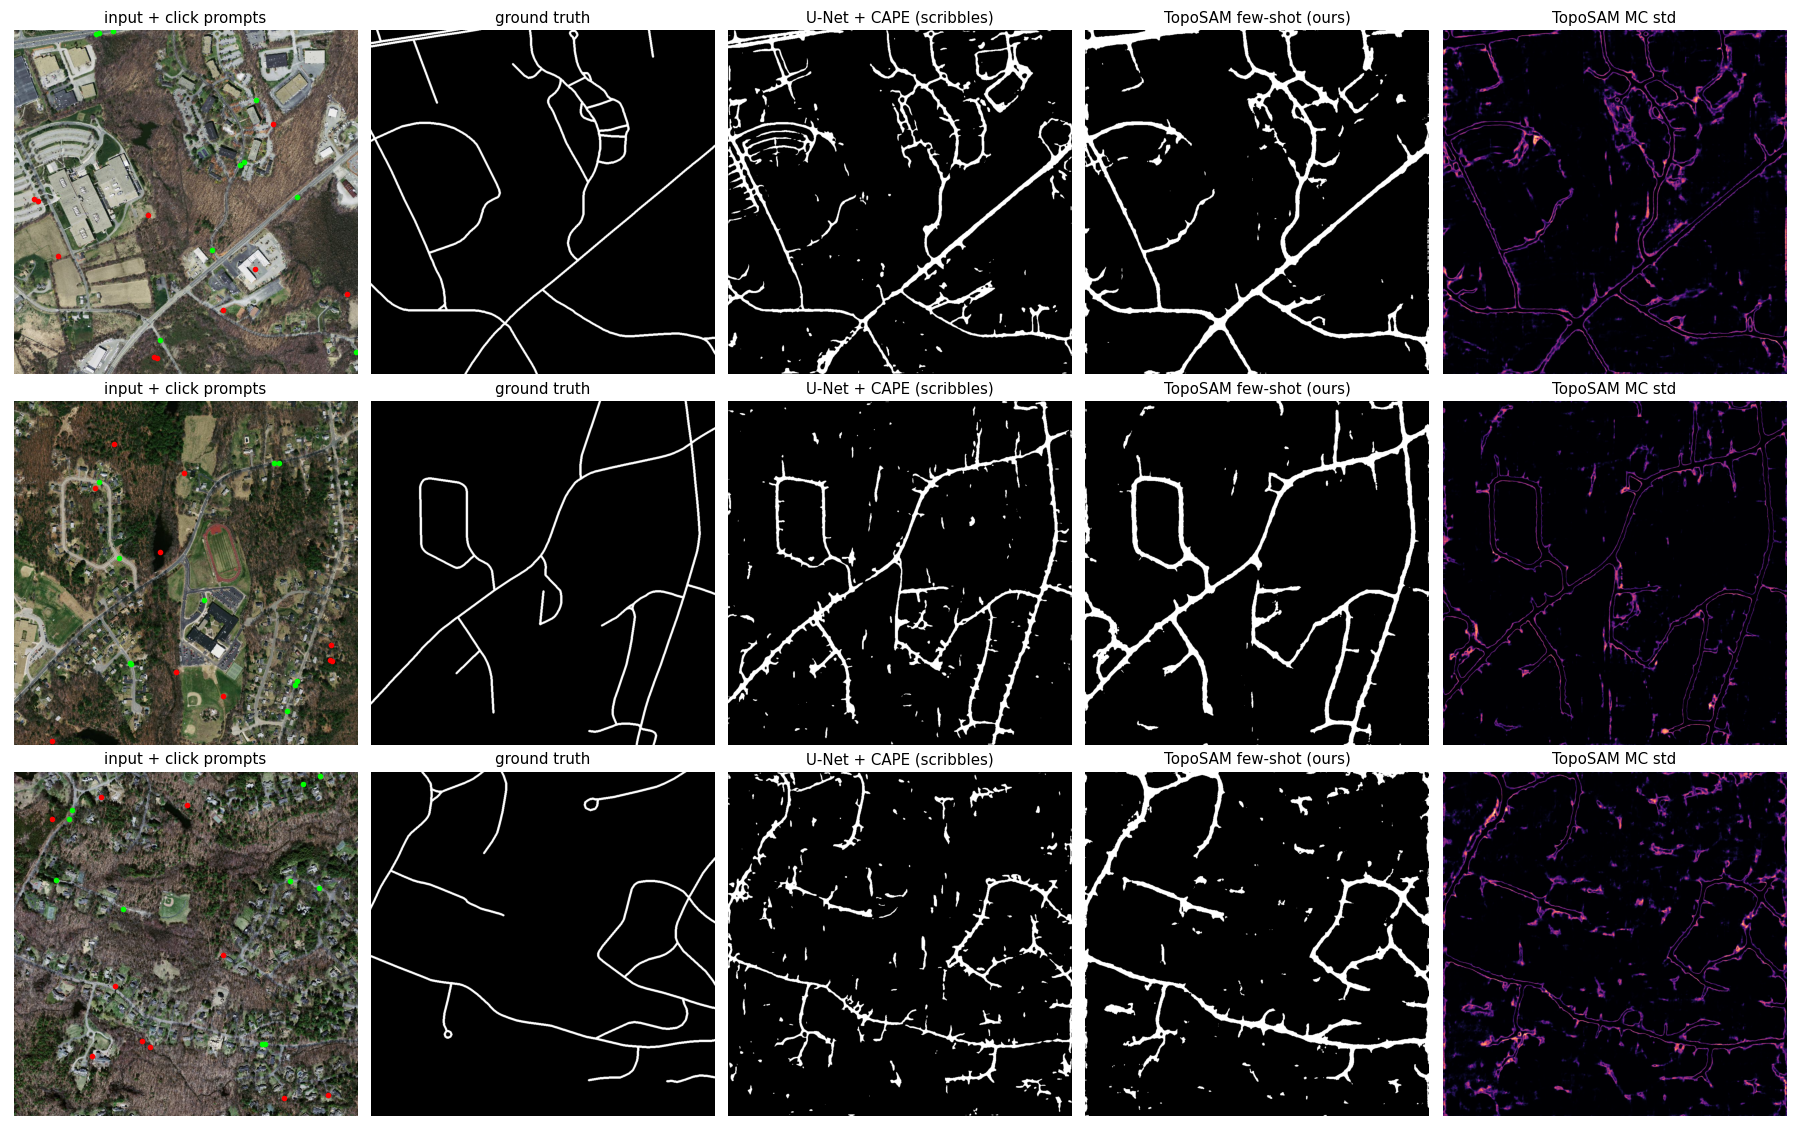
\includegraphics[width=0.78\textwidth]{figures/qual_roads.png}
\caption{Few-shot roads (40 tiles with scribbles). Columns: input with the click prompts (green positive, red negative), ground truth, U-Net + CAPE, TopoSAM, TopoSAM MC standard deviation.}\label{fig:roads}
\end{figure*}

% Auto-generated by gen_paper_assets.py; do not edit by hand.
\begin{table}[t]
\centering\caption{Zero-shot vessel$\to$road transfer without road labels (30 test tiles). $s$ is the test-time rescaling; the scale-space ridge estimate gives $s=0.72$.}\label{tab:zeroshot}
\setlength{\tabcolsep}{2pt}\scriptsize\begin{tabular}{llccc}\toprule
Model & Test-time input & Dice & clDice & $\beta_0$ err.\\\midrule
TopoSAM-DRIVE + polarity aug. & as is, $s$=1 & 0.205 & 0.187 & 6.77\\
 & as is, $s$=0.5 & 0.170 & 0.167 & 1.89\\
 & inverted, $s$=0.5 & 0.369 & 0.370 & 1.81\\
 & polarity ensemble, $s$=0.5 & 0.357 & 0.391 & 1.24\\
 & min.\ entropy per tile & 0.220 & 0.197 & 5.85\\
+ RandConv texture aug. & as is, $s$=0.5 & 0.297 & 0.297 & 2.04\\
 & inverted, $s$=0.5 & 0.324 & 0.321 & 2.17\\
 & polarity ensemble, $s$=0.5 & 0.351 & 0.373 & 1.38\\
\bottomrule\end{tabular}\end{table}

\subsection{Zero-Shot Vessel-to-Road Transfer}
Without road labels, every vessel model fails on roads (clDice \NZSBase{} for TopoSAM). Table~\ref{tab:zeroshot} diagnoses why: vessels are dark lines and roads bright ones, and roads are about twice as wide. Inverting intensities and halving the scale doubles clDice; averaging both polarities, which needs no knowledge of the polarity, gives \NZSBest. Training with random-convolution textures and inverted copies makes the model polarity-invariant (as-is input at half scale: \NZSPolRaw{}$\to$\NZSTexRaw{}; gap between polarities 0.20$\to$0.02) but does not raise the best score, which is limited by the remaining fundus-to-aerial domain gap.

\FloatBarrier
\section{Limitations and Negative Results}\label{sec:disc}
\textbf{What did not work.} (i) Selecting the polarity and scale per image without labels failed: a scale-space Hessian ridge test \cite{frangi1998,lindeberg1998} gives the right scale direction (0.72$\times$) but an ambiguous polarity, because the background between two lines is itself a ridge of the opposite polarity; per-tile minimum-entropy selection \cite{tent} prefers confidently \emph{empty} predictions (clDice 0.20). Averaging polarities is the rule that works. (ii) The texture-randomised initialisation helps zero-shot transfer but slightly hurts few-shot fine-tuning ($-0.018$ clDice). (iii) The diversity radius chosen on validation ($r=48$) is not better than $r=24$ on test. (iv) A noisy annotator costs about 0.075 clDice. (v) CRC is infeasible for $\alpha<0.06$ with 16 calibration images.
\textbf{Scope.} Datasets are small (20 DRIVE test images, 60 road tiles) and two-dimensional; three seeds give limited precision on variance; Wilcoxon tests use images as the unit and do not measure variability over training sets. Annotations for weak supervision are simulated. Our connectivity is local (pairs up to 30 pixels apart in a $64^2$ tile); long-range connectivity is not certified. Stronger baselines---structure-level uncertainty \cite{gupta2023}, nnU-Net backbones, more datasets and 3-D volumes---are the next step.

\section{What This Changes in Practice}\label{sec:impact}
Topology-aware losses improve the expected connectivity of a map; conformal connectivity tells the user which connections to trust in \emph{this} map. In a review workflow the guarantee translates directly into workload: on CAPE models, a reviewer inspects about a third of the connections and is shown roughly three quarters of all topology errors, with a provable bound on the rest. The same score makes topology-aware training cheaper, by asking annotators the yes/no questions that matter instead of tracing every vessel.

\section{Conclusion}
We made connectivity the unit of uncertainty for curvilinear segmentation. A widest-path characterisation of thresholded connectivity, combined with MC-dropout, yields a connection score that detects topology errors; conformal prediction and an image-level risk-control theorem turn it into calibrated, provable decisions; and the same score drives label-efficient training of CAPE and of a CAPE-trained Segment-Anything model. The method is compatible with any topology-aware loss and adds a missing layer to them: not only connected predictions, but connections one can trust.

\section*{Acknowledgments}
We thank the authors of CAPE for releasing their implementation under the MIT license, and the providers of the DRIVE and Massachusetts Roads datasets.

\section*{Statements and Declarations}
\noindent\textbf{Funding.} No funds, grants, or other support were received for this study.\par
\noindent\textbf{Competing interests.} The author declares no relevant financial or non-financial competing interests.\par
\noindent\textbf{Ethics approval and consent.} Not applicable; only public, de-identified datasets were used.\par
\noindent\textbf{Data availability.} DRIVE and Massachusetts Roads are publicly available. Summary results and the scripts that regenerate every table, number and figure of this paper are available at \url{https://github.com/Youssef-Ahmed38/conformal-connectivity-cape}; trained models and per-pair caches are regenerated by the scripts.\par
\noindent\textbf{Code availability.} All source code (training, connection score, guarantees, label-efficient CAPE, TopoSAM, exact parallel CAPE) and tests are available at \url{https://github.com/Youssef-Ahmed38/conformal-connectivity-cape} under the MIT license.\par
\noindent\textbf{Author contributions.} Y.~Mourad conceived and designed the study, developed the methods and software, performed the experiments, analysed the data, and wrote the manuscript.\par

\balance
\begin{thebibliography}{40}
\bibitem{cldice} S. Shit, J. C. Paetzold, A. Sekuboyina, I. Ezhov, A. Unger, A. Zhylka, J. P. W. Pluim, U. Bauer, and B. H. Menze, ``clDice---a novel topology-preserving loss function for tubular structure segmentation,'' in \emph{Proc.\ IEEE/CVF Conf.\ Computer Vision and Pattern Recognition (CVPR)}, 2021.
\bibitem{hu2019} X. Hu, F. Li, D. Samaras, and C. Chen, ``Topology-preserving deep image segmentation,'' in \emph{Advances in Neural Information Processing Systems (NeurIPS)}, 2019.
\bibitem{stucki2023} N. Stucki, J. C. Paetzold, S. Shit, B. Menze, and U. Bauer, ``Topologically faithful image segmentation via induced matching of persistence barcodes,'' in \emph{Proc.\ Int.\ Conf.\ Machine Learning (ICML)}, 2023.
\bibitem{cape} E. Esmaeilzadeh, E. Garaaghaji, F. Hallaji Azad, and D. Oner, ``CAPE: Connectivity-aware path enforcement loss for curvilinear structure delineation,'' in \emph{Medical Image Computing and Computer Assisted Intervention (MICCAI)}, 2025, arXiv:2504.00753.
\bibitem{mosinska2018} A. Mosinska, P. M\'arquez-Neila, M. Kozi\'nski, and P. Fua, ``Beyond the pixel-wise loss for topology-aware delineation,'' in \emph{Proc.\ IEEE/CVF Conf.\ Computer Vision and Pattern Recognition (CVPR)}, 2018.
\bibitem{oner2022} D. Oner, M. Kozi\'nski, L. Citraro, N. C. Dadap, A. G. Konings, and P. Fua, ``Promoting connectivity of network-like structures by enforcing region separation,'' \emph{IEEE Trans.\ Pattern Analysis and Machine Intelligence}, 2022.
\bibitem{mosinska2017} A. Mosinska, J. Tarnawski, and P. Fua, ``Active learning and proofreading for delineation of curvilinear structures,'' in \emph{Medical Image Computing and Computer Assisted Intervention (MICCAI)}, 2017.
\bibitem{gupta2023} S. Gupta, Y. Zhang, X. Hu, P. Prasanna, and C. Chen, ``Topology-aware uncertainty for image segmentation,'' in \emph{Advances in Neural Information Processing Systems (NeurIPS)}, 2023.
\bibitem{gal2016} Y. Gal and Z. Ghahramani, ``Dropout as a Bayesian approximation: Representing model uncertainty in deep learning,'' in \emph{Proc.\ Int.\ Conf.\ Machine Learning (ICML)}, 2016.
\bibitem{lakshminarayanan2017} B. Lakshminarayanan, A. Pritzel, and C. Blundell, ``Simple and scalable predictive uncertainty estimation using deep ensembles,'' in \emph{Advances in Neural Information Processing Systems (NeurIPS)}, 2017.
\bibitem{guo2017} C. Guo, G. Pleiss, Y. Sun, and K. Q. Weinberger, ``On calibration of modern neural networks,'' in \emph{Proc.\ Int.\ Conf.\ Machine Learning (ICML)}, 2017.
\bibitem{zadrozny2002} B. Zadrozny and C. Elkan, ``Transforming classifier scores into accurate multiclass probability estimates,'' in \emph{Proc.\ ACM SIGKDD Int.\ Conf.\ Knowledge Discovery and Data Mining}, 2002.
\bibitem{vovk2005} V. Vovk, A. Gammerman, and G. Shafer, \emph{Algorithmic Learning in a Random World}. Springer, 2005.
\bibitem{angelopoulos2021} A. N. Angelopoulos and S. Bates, ``A gentle introduction to conformal prediction and distribution-free uncertainty quantification,'' arXiv:2107.07511, 2021.
\bibitem{crc} A. N. Angelopoulos, S. Bates, A. Fisch, L. Lei, and T. Schuster, ``Conformal risk control,'' in \emph{Int.\ Conf.\ Learning Representations (ICLR)}, 2024.
\bibitem{tibshirani2019} R. J. Tibshirani, R. Foygel Barber, E. J. Cand\`es, and A. Ramdas, ``Conformal prediction under covariate shift,'' in \emph{Advances in Neural Information Processing Systems (NeurIPS)}, 2019.
\bibitem{mossina2025} L. Mossina and C. Friedrich, ``Conformal prediction for image segmentation using morphological prediction sets,'' arXiv:2503.05618, 2025.
\bibitem{kervadec2019} H. Kervadec, J. Dolz, M. Tang, E. Granger, Y. Boykov, and I. Ben Ayed, ``Constrained-CNN losses for weakly supervised segmentation,'' \emph{Medical Image Analysis}, 2019.
\bibitem{randconv} Z. Xu, D. Liu, J. Yang, C. Raffel, and M. Niethammer, ``Robust and generalizable visual representation learning via random convolutions,'' in \emph{Int.\ Conf.\ Learning Representations (ICLR)}, 2021.
\bibitem{sam} A. Kirillov, E. Mintun, N. Ravi, H. Mao, C. Rolland, L. Gustafson, T. Xiao, S. Whitehead, A. C. Berg, W.-Y. Lo, P. Doll\'ar, and R. Girshick, ``Segment anything,'' in \emph{Proc.\ IEEE/CVF Int.\ Conf.\ Computer Vision (ICCV)}, 2023.
\bibitem{dijkstra} E. W. Dijkstra, ``A note on two problems in connexion with graphs,'' \emph{Numerische Mathematik}, vol. 1, pp. 269--271, 1959.
\bibitem{drive} J. Staal, M. D. Abr\`amoff, M. Niemeijer, M. A. Viergever, and B. van Ginneken, ``Ridge-based vessel segmentation in color images of the retina,'' \emph{IEEE Trans.\ Medical Imaging}, vol. 23, no. 4, 2004.
\bibitem{mnih2013} V. Mnih, ``Machine learning for aerial image labeling,'' Ph.D.\ dissertation, University of Toronto, 2013.
\bibitem{unet} O. Ronneberger, P. Fischer, and T. Brox, ``U-Net: Convolutional networks for biomedical image segmentation,'' in \emph{Medical Image Computing and Computer Assisted Intervention (MICCAI)}, 2015.
\bibitem{wilcoxon} F. Wilcoxon, ``Individual comparisons by ranking methods,'' \emph{Biometrics Bulletin}, vol. 1, no. 6, pp. 80--83, 1945.
\bibitem{frangi1998} A. F. Frangi, W. J. Niessen, K. L. Vincken, and M. A. Viergever, ``Multiscale vessel enhancement filtering,'' in \emph{Medical Image Computing and Computer Assisted Intervention (MICCAI)}, 1998.
\bibitem{lindeberg1998} T. Lindeberg, ``Edge detection and ridge detection with automatic scale selection,'' \emph{Int.\ J.\ Computer Vision}, vol. 30, no. 2, 1998.
\bibitem{tent} D. Wang, E. Shelhamer, S. Liu, B. Olshausen, and T. Darrell, ``Tent: Fully test-time adaptation by entropy minimization,'' in \emph{Int.\ Conf.\ Learning Representations (ICLR)}, 2021.
\end{thebibliography}
\end{document}
